\documentclass[11pt,a4paper]{report} 
\usepackage[utf8]{inputenc}%encodage
\usepackage[T1]{fontenc}%accens
\usepackage[french]{babel}%français
%\usepackage{arev}%police
\usepackage[top=2.5cm,bottom=2.5cm,left=2.5cm,right=2.5cm]{geometry}
\frenchbsetup{StandardLists=true}
\usepackage{multicol}
\usepackage{shapepar}
\usepackage{nccrules}
\usepackage{ulem}
\usepackage{appendix}
\usepackage[squaren]{SIunits}
\usepackage{shorttoc}
\usepackage{eurosym}
\usepackage{color}
\usepackage{graphicx}
\usepackage{float}
\usepackage{wrapfig}
\usepackage{caption}
\usepackage{amsmath}
\usepackage{amssymb}
\usepackage{subfigure}
\setlength{\columnsep}{1cm}
\setlength{\parindent}{0pt}
\setlength{\columnseprule}{0pt}
\usepackage{fancyhdr}
\pagestyle{fancy}
\usepackage{array}
\usepackage{pgfgantt}
\usepackage{enumitem}
\usepackage{geometry}
\usepackage{multirow}
\usepackage{vmargin}

\parindent=0cm
\pagestyle{plain}
\usepackage{hyperref}

\begin{document}

\begin{titlepage}

\newcommand{\HRule}{\rule{\linewidth}{0.5mm}} % Defines a new command for the horizontal lines, change thickness here

\center % Center everything on the page
 
%----------------------------------------------------------------------------------------
%	HEADING SECTIONS
%----------------------------------------------------------------------------------------

\textsc{\LARGE ESAIP école d'ingénieur}\\[1.5cm] % Name of your university/college

\includegraphics[scale=0.5]{logo_esaip}\\[1cm] % Include a department/university logo - this will require the graphicx package
\textsc{\Large Dossier de spécifications}\\[0.5cm] % Major heading such as course name
\textsc{\large Projet Appliatif}\\[0.5cm] % Minor heading such as course title

%----------------------------------------------------------------------------------------
%	TITLE SECTION
%----------------------------------------------------------------------------------------

\HRule \\[0.4cm]
{ \huge \bfseries Annuaire ESAIP}\\[0.4cm] % Title of your document
\HRule \\[1.5cm]
 
%----------------------------------------------------------------------------------------
%	AUTHOR SECTION
%----------------------------------------------------------------------------------------

\begin{minipage}{0.4\textwidth}
\begin{flushleft} \large
\emph{\textbf {Author:}}\\
Baptiste \textsc{DEVES}\\ % Your name
Jordan \textsc{FRAUD-GELDOF}\\
Nicolas \textsc{GAUME}\\
Alexandre \textsc{JOURDOIS}\\
Nicolas \textsc{PIRON}\\
\end{flushleft}

\end{minipage}\\[2cm]

% If you don't want a supervisor, uncomment the two lines below and remove the section above
%\Large \emph{Author:}\\
%John \textsc{Smith}\\[3cm] % Your name

%----------------------------------------------------------------------------------------
%	DATE SECTION
%----------------------------------------------------------------------------------------

{\large \today}\\[2cm] % Date, change the \today to a set date if you want to be precise

\vfill % Fill the rest of the page with whitespace

\end{titlepage}
%renommer la table des matières en sommaire
\renewcommand{\contentsname}{Sommaire} 
%table des matières (position)
\tableofcontents

%\part{Partie 1}
	\chapter{Rappels sur le projet}
		De notre temps les avancés technologiques sont infinies, à l'inverse des ressources de notre planète. C'est dans le but préserver notre environnement que le green IT à vu le jour dans les année 90. Divers manifestations dans ce domaine ont été créées pour sensibiliser les populations mais surtout les techniciens et ingénieurs de demain à la conception éco-responsable. Cette année le GreenIT a permis à différentes écoles de France et d'Europe de constituer des équipes de 5 personnes et de se rencontrer dans une compétition  où la récompense était offerte à ceux qui réaliserait l'application web la plus green et avec la meilleure expérience utilisateur. Le défis de cette année était de réaliser une application web d'annuaire de dentistes. Dans la continuité du Design4Green nous avons décidé de réaliser un annuaire adapté à l'ESAIP.
		
	\chapter{Spécifications fonctionnelles}
		\section{Objectifs}
		Le but de cette application web est de pouvoir aider tous les interlocuteurs de l'ESAIP à résoudre leurs problèmes en trouvant à qui s'adresser. Trouver une salle disponible pour travailler ne sera plus un problème quand nous pourrons avoir accès à tous les emplois du temps des salles et leurs disponibilités en temps réel. D'autre part nous avons pour objectif de créer un site respectueux de l'environnement. 
		\section{Acteurs} 
		Par expérience nous savons qu'il n'est pas chose facile d'arriver dans un nouvel établissement. Ne pas connaître les professeurs, le personnel administratif ou même les autres étudiants peut être un frein à la résolution de certains problèmes ou même à l'avancée de certaines démarches. Ce service sera donc disponible aux acteurs ci-dessous :
			\begin{itemize}
				\item Admin (résolution des problèmes du site)
				\item Clients
					\begin{itemize}
						\item Elèves
						\item Professeurs
						\item Personnels administratifs
					\end{itemize}
			\end{itemize}
		\section{Fonctionnalités}
			Fonctionnalités offertes par le service :
				\begin{enumerate}
					\item Obtenir des informations sur le site:
							\begin{itemize}
								 \item Publications de l'administrateur, mise à jour des profiles, mentions légales
								 \item Contacter l'administrateur en cas de problème
							\end{itemize}
					\item Trouver des informations sur :
				\begin{itemize}
					\item une personne 
										\begin{itemize}
											\item en rapport avec son domaine de compétence
											\item afficher son nom, prénom, son poste, l'emplacement de son bureau, une photo
										\end{itemize}
					\item une salle 
										\begin{itemize}
											\item l'emploi du temps de cette salle
											\item sa disponibilité en temps réel
										\end{itemize}
					\end{itemize}
				\end{enumerate}
				\begin{center}
					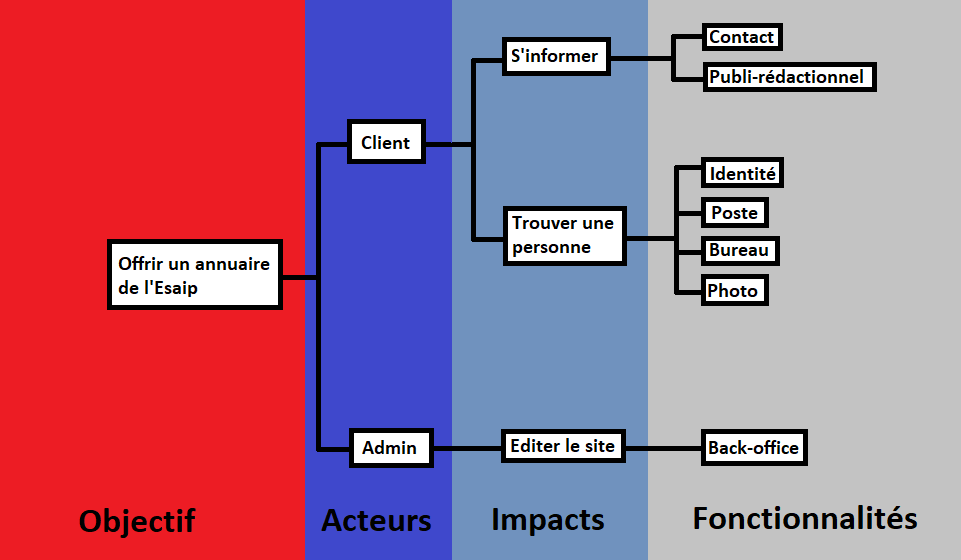
\includegraphics[scale=0.43]{OAIF}
				\end{center}
				
	\chapter{Spécifications générales}
		\section{Présentation de l'application web}
            \subsection{Environnement de l'application web}
            	Notre application web sera hébergée sur un VPS, nous allons mettre en place un serveur web lighttpd et nous utiliserons comme langage de programmation l’angular js pour l’application.
            \subsection{Description de l'application web}
            	L’objectif du projet est de mettre en place un annuaire de l’ESAIP qui permet de retrouver des personnes internes à l’école. Les principales fonctions à mettre en place seront :   
            	\begin{itemize}
            		\item Une base de données complète.
            		\item Une fonction de recherche polyvalente pour trouver une personne.
            		\item Une fonction de recherche de salle libre.
            		\item Un plan de l’école indiquant les différentes salles/bureaux.
				\end{itemize}
				            				
		\section{Contraintes de réalisation}
			\subsection{Contraintes d'évolution}
				Si l’on pense à l’avenir, nous souhaiterions que notre application Web puisse être améliorée par la suite, qu’elle reste à jour et qu’elle soit adaptée en application pour Smartphones. C’est dans cette optique que nous allons essayer de structurer notre programme le plus clairement possible et que nous voudrions trouver des successeurs afin de gérer les mises à jour de la base de données.		
			\subsection{Contraintes de développement}
				Afin de rester sur une application légère nous avons pour contrainte d’utiliser des technologies légères qui n’utilisent pas trop de ressources. Pour l’instant nous avons choisi de travailler en angular js pour le back-end et html/css/js pour le front-end, mais ces technologies pourraient évoluer au cours du projet si nous découvrons une façon plus green de réaliser notre application web.	
			\subsection{Contraintes de qualité}  
				Nous avons considéré comme critères de qualités principaux pour évaluer notre projet :
				
				\begin{itemize}
            		\item L’expérience utilisateur
            		\item Les ressources consommées
				\end{itemize}
				
	\chapter{Spécifications d'interface}
		\section{Interface web}
		Toutes les images présente dans ce paragraphe sont à titre schématique, l'esthétique final peut évoluer. L'en-tête sera la même pour toutes les pages, un logo de l'ESAIP, un bandeau "Annuaire" et des onglets L'en-tête sera la même pour toutes les pages, un logo de l'ESAIP, un bandeau "Annuaire" et des onglets (Accueil, Contact, Mentions légales).A.
L'onglet Accueil permettra un retour à la page principale, Contact renvoie sur la page de contact et Mentions légales renvoie sur la page éponymes.
			\begin{center}
					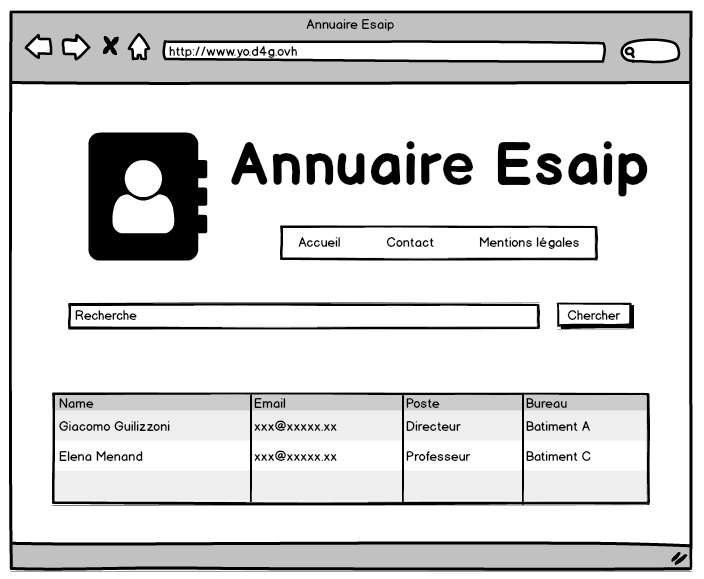
\includegraphics[scale=0.4]{site}
			\end{center}
			Dans un souci de rapidité de réponse pour l'utilisateur, la page d'Accueil ne supporte que quelques éléments : l'en-tête, un bandeau de recherche, un bouton et la liste des personnes correspondant à la recherche.
Le bandeau de recherche intégrera une fonction d'auto-complétion/proposition dès 3 caractères tapés, correspondant à toutes informations d'une personne : si l'utilisateur tape "jou" l'étudiant Jourdois Alexandre peut être proposé directement.
Le bouton "Chercher" lance la recherche dans la base de données. Enfin, une liste de personne découle de la recherche, avec quelques informations. Si l'utilisateur clique sur une identité, la page du contact s'affiche.
			\begin{center}
					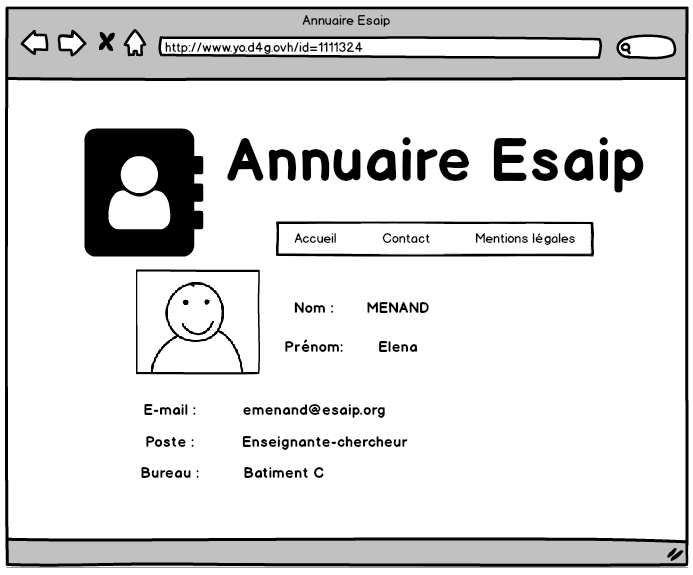
\includegraphics[scale=0.4]{site2}
			\end{center}
			La page contact renvoie une fiche d'identité du contact sélectionné précédemment. Informations affichées : nom, prénom, e-mail, poste/filière, bureau.
			\begin{center}
					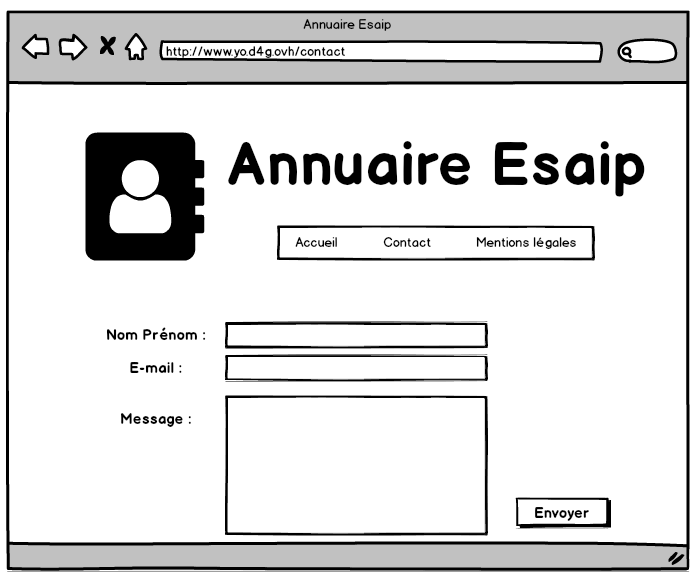
\includegraphics[scale=0.4]{site3}
			\end{center}
			
			La page Contacter renvoie un formulaire de contact pour l'utilisateur, afin de contacter le service d'administration pour une question ou un problème. L'utilisateur doit finir son nom et prénom, son e-mail et le message à envoyer. Un bouton "Envoyer" permet l'envoi du message une fois les champs complétés.
			\begin{center}
					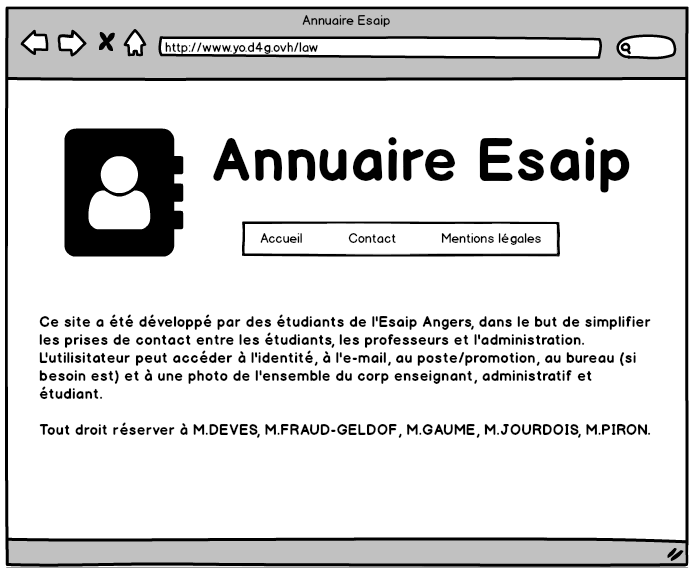
\includegraphics[scale=0.4]{site4}
			\end{center}
			La page Mentions Légales pose le cadre de cette application web et son fonctionnement, ainsi que les auteurs de cette application.
			\subsection{Architecture du site}
			\begin{center}
				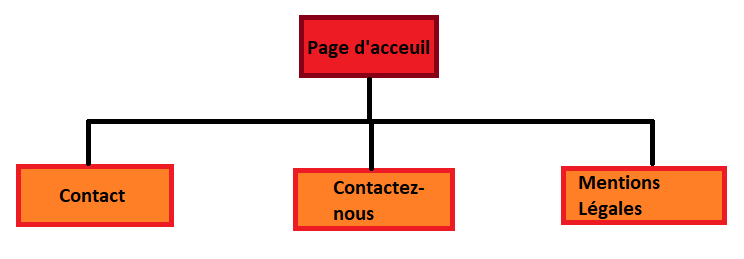
\includegraphics[scale=0.55]{structure}
			\end{center}
			\subsection{Contraintes d'utilisation de l'interface}
				 L'utilisation du serveur fournit suite au challenge du design4green, nous limites sur le nombre de requêtes que le site peut recevoir par l'utilisateur. Une connexion simultanée de tous les utilisateurs est fortement déconseillée.
		
\end{document}

